\documentclass[sigconf]{acmart}
\usepackage{booktabs}
\usepackage{xurl}
\usepackage{tikz}
\usetikzlibrary{positioning,arrows.meta,fit}
\settopmatter{printacmref=false}
\setcopyright{none}
\renewcommand\footnotetextcopyrightpermission[1]{}
\acmConference[RL4LLM-Agents '26]{Workshop on Reinforcement Learning for LLM-based Agents at ICAIF 2026}{November 14--15, 2026}{Milan, Italy}
\acmYear{2026}
\acmDOI{}
\acmISBN{}

\begin{document}

\title{Which Outcome Should Teach an LLM Reader?}
\subtitle{A Verified FOMC Benchmark and Reward-Design Evidence for Outcome-Guided Agents in Finance}

\author{Manuel Bossi}
\affiliation{%
  \institution{Stevens Institute of Technology}
  \city{Hoboken}
  \state{New Jersey}
  \country{USA}}
\email{mbossi@stevens.edu}

\renewcommand{\shortauthors}{M. Bossi}
\setlength{\emergencystretch}{1.5em}

\begin{abstract}
Harness-side learning methods such as reflection and prompt evolution let an LLM agent improve from outcome feedback without updating its weights. In finance the natural feedback is a market or policy outcome, and such an outcome is a useful reward only when the documents the agent reads carry learnable information about it. We report a verified benchmark for outcome-guided reading of Federal Open Market Committee (FOMC) minutes, built on Cieslak and Vissing-Jorgensen's study of the ``Fed put,'' the Federal Reserve's tendency to ease policy after poor stock-market performance. The benchmark contains 1,197 equity-market passages from the minutes of 200 meetings (2000--2024), fixed chronological splits, an audited reconstruction of the authors' automated phrase-and-direction method, and the authors' human-coded tone counts, which we recover from their published figures. Screening two candidate rewards with frozen readers, whose models and instructions stay fixed, gives opposite answers. The equity return that preceded a meeting is learnable from the minutes. A frozen embedding recovers it with an out-of-sample $R^2$ of 0.50, and tone labels from a frozen LLM reach 0.49, against 0.32 for a linear readout of the reconstructed phrase-and-direction counts. The next change in the policy rate shows no detectable signal. In a test specified before estimation, no text representation beats a baseline without text. A pilot with a frozen LLM reader exposes a credit-assignment problem. One crisis meeting accounts for 79\% of the pilot's feedback error, although the reader labels all of its passages negative, which is the correct direction. An LLM reflector that rewrites the reader's instructions from outcome residuals would therefore be pushed to change labels whose direction is already right. We release the environment, the comparators, and a validation-gated adaptation protocol. We have not yet run the adaptive comparisons.
\end{abstract}

\begin{CCSXML}
<ccs2012>
<concept><concept_id>10010147.10010178.10010179</concept_id><concept_desc>Computing methodologies~Natural language processing</concept_desc><concept_significance>500</concept_significance></concept>
<concept><concept_id>10010405.10010455.10010460</concept_id><concept_desc>Applied computing~Economics</concept_desc><concept_significance>300</concept_significance></concept>
</ccs2012>
\end{CCSXML}
\ccsdesc[500]{Computing methodologies~Natural language processing}
\ccsdesc[300]{Applied computing~Economics}

\keywords{LLM agents, reward design, reflection, validation gates, central-bank communication, FOMC minutes, benchmark}

\maketitle

\section{Introduction}

Reflection~\cite{shinn2023reflexion}, LLM-driven prompt optimization~\cite{yang2024opro}, and reflective prompt evolution~\cite{agrawal2025gepa} improve an agent by editing its instructions or memory in response to scored outcomes. These methods move the design burden from the optimizer to the reward. A reward that is noisy, unlearnable from the agent's inputs, or silent about which intermediate step failed will still produce edits, and a persistent memory will keep them.

Financial document reading makes the problem concrete. An agent that reads central-bank minutes can be scored against observable outcomes: the market move the minutes describe, the market's reaction to their release, or the next policy decision. These outcomes are exact and need no LLM judge. They differ sharply in whether the text contains information about them, and an agent cannot tell the difference from a single residual.

We build and verify a benchmark for this setting and use it to screen rewards before any agent is adapted. The environment pairs FOMC minutes with the measures of Cieslak and Vissing-Jorgensen~\cite{cvj2021,cvj2020}, who study the ``Fed put,'' the tendency of the Federal Reserve to ease policy after poor stock-market performance. They count mentions of the stock market in the minutes, code the tone of each mention by hand, and relate these measures to returns and policy; an automated phrase-and-direction algorithm provides their robustness checks. We reconstruct that algorithm, recover their human-coded counts from the published figures, and evaluate every reader on the same chronological splits.

The paper makes four contributions:
\begin{itemize}
\item \textbf{A verified environment.} We release episodes, passages, targets, folds, and fixed comparators, including the recovered human coding, with a SHA-256 hash for every input (\S\ref{sec:env}).
\item \textbf{Reward screening.} Frozen readers show that the preceding return is a learnable reward and that the next policy change, tested under a protocol fixed before estimation, offers no detectable text signal (\S\ref{sec:screen}).
\item \textbf{A credit-assignment diagnostic.} In a pilot, most of the outcome error comes from one episode whose passages the reader labels in the correct direction, so outcome residuals do not locate reading errors (\S\ref{sec:credit}).
\item \textbf{An adaptation protocol and its cost.} Holding out feedback and gate meetings from calibration raises the mean squared error (MSE) of the strongest frozen reader by 15.7\% before any adaptation. We specify a validation-gated protocol and the fixed-reader baseline that any adaptive arm must beat (\S\ref{sec:protocol}).
\end{itemize}
We have not yet run the adaptation arms, so the paper reports no learning results.

\section{Related work}

\textbf{Harness-side learning.} Reflexion stores verbal self-feedback in episodic memory~\cite{shinn2023reflexion}. OPRO uses an LLM to propose instructions scored by task accuracy~\cite{yang2024opro}, and GEPA evolves prompts from execution traces with Pareto selection~\cite{agrawal2025gepa}. Our readers are compatible with all three. We ask which financial outcome such a harness-side learning loop should optimize.

\textbf{Outcome versus process feedback.} Outcome-only feedback can reward correct answers reached for the wrong reasons, and step-level supervision can improve reliability~\cite{uesato2022process,lightman2024verify}. Optimizing a proxy reward can also degrade the true objective~\cite{skalse2022reward}. Our credit-assignment case is a financial instance of the gap between outcome and process supervision.

\textbf{Text and central-bank communication.} Text-as-data methods in economics~\cite{gentzkow2019text} increasingly use LLMs for central-bank language~\cite{hansen2023fedspeak,gambacorta2024cblm}. Ludwig et al.~\cite{ludwig2026} distinguish LLMs used for measurement from LLMs used for prediction. Repeated model selection on the same validation data biases performance estimates upward~\cite{cawley2010}, and iterative harness adaptation repeats that selection many times.

\section{Environment}\label{sec:env}

\textbf{Episodes and observations.} An episode is one FOMC meeting. The corpus holds the minutes of 200 meetings from February 2000 to December 2024, and 199 of them have a return target. Sixteen fixed equity-market phrase patterns, separate from the comparator's dictionary described below, match 1,314 text segments. Each match, together with one neighboring segment on either side, forms a passage, and deduplication leaves 1,197 unique passages. The reader sees only the meeting's passages, in document order. Dates, identifiers, and targets are visible only to the evaluator.

\textbf{Actions and readout.} A reader assigns each passage one of five tone categories (positive, negative, neutral, hypothetical, unclear) with exact supporting quotations. A deterministic aggregator counts categories by meeting, and a ridge readout maps the counts and document length to the target. The ridge penalty is chosen by chronological inner validation, with every transformation fitted on training meetings only. A continuous alternative replaces the counts with the meeting mean of L2-normalized 3,072-dimensional passage embeddings~\cite{lee2025gemini}.

\textbf{Formal setup.} Meeting $m$ supplies an ordered passage set $T_m=(t_{m1},\dots,t_{mJ_m})$ and document length $L_m$. A reader with instructions and memory $g$ maps each passage to a category and evidence, $a_{mj}=\pi_g(t_{mj})$. The aggregator forms counts $c_m(g)\in\mathbb N^5$, and a readout $h$ fitted on calibration meetings $C$ (the full training window for the frozen benchmark, and its oldest 60\% in the adaptive protocol of \S\ref{sec:protocol}) gives $\hat y_m(g)=h_{g,C}(c_m(g),L_m)$. The episode reward is
\begin{equation}\label{eq:reward}
r_m(g)=-\bigl(y_m-\hat y_m(g)\bigr)^2 ,
\end{equation}
one scalar per meeting, regardless of how many passages the meeting contains. For a reward target $y$, a family $\mathcal K$ of frozen readers, and a baseline readout $b$ that uses no passage content (document length alone for recovery, the controls for policy), we define the \emph{headroom} of $y$ as
\begin{equation}\label{eq:headroom}
H(y)=1-\frac{\min_{k\in\mathcal K}\mathrm{MSE}_E(k)}{\mathrm{MSE}_E(b)},
\end{equation}
measured on the untouched evaluation meetings $E$. Harness adaptation searches over $g$ only; model weights, retrieval, the category set, the aggregator, and the readout family stay fixed. If $H(y)\le 0$ for a family that includes strong frozen readers, the reward can teach an adaptive reader only the noise in its training meetings.

\textbf{Targets.} The \emph{recovery} target is the S\&P 500 price return over the intermeeting period, from the day after the previous meeting to two days before the current one, in excess of the three-month Treasury bill rate. The return is realized before the minutes are written, so recovering it measures how well a reader interprets the text. The \emph{policy} target is the change in the federal funds target rate (after December 2008, the midpoint of the target range) from the day after meeting $m$ to the day after meeting $m+1$. The policy regressions control for document length, the target level and its change around meeting $m$, and the negative and positive parts of the returns before meeting $m$ and over the following intermeeting period.

\textbf{Splits.} The first 100 labeled meetings initialize training. The remaining 99 form five expanding-window evaluation blocks (folds 0--4), with refits at September 2012, March 2015, September 2017, March 2020, and September 2022. The policy task uses the same boundaries and has 98 evaluation meetings, because the last meeting has no successor.

\textbf{Comparators.} We reimplement the published phrase-and-direction algorithm (47 noun patterns and 93 direction patterns, with adjacency, negation, and clause-boundary rules) and audit it against 24 constructed tests. We also recover the original human-coded counts and return series from the vector graphics of the published figures. The recovered counts match the printed totals exactly (975 stock-market mentions, of which 322 are coded negative and 414 positive) and agree across two independent figures for all 184 meetings of the original 1994--2016 sample. The human counts serve only as evaluation references and never enter an agent's feedback. Table~\ref{tab:card} summarizes the environment and Table~\ref{tab:bench} the frozen-reader results.

\begin{table}[t]
\caption{Benchmark card.}
\label{tab:card}
\small
\begin{tabular}{@{}p{0.27\linewidth}p{0.66\linewidth}@{}}
\toprule
Episodes & 199 labeled FOMC meetings, Mar 2000--Dec 2024 (one reward each) \\
Observations & 1,197 unique equity-market passages from the minutes of 200 meetings, about 6 per meeting \\
Actions & 5 tone categories + exact evidence quotes per passage \\
Rewards & Recovery of preceding excess return, in percentage points (pp); next-cycle target change, in basis points (bp) \\
Splits & 100 initial training meetings; 5 expanding blocks with 99 evaluation meetings (98 for policy) \\
Comparators & Length only; TF--IDF (term frequency--inverse document frequency); reconstructed rules (linear, quadratic); frozen embedding; LLM tone counts; recovered human counts (35-meeting overlap) \\
Checks & SHA-256 for every document and market file; 24 rule tests; exact reproduction of published totals; hashed policy protocol \\
\bottomrule
\end{tabular}
\end{table}

\begin{table}[t]
\caption{Frozen readers on the recovery reward, 99 evaluation meetings. RMSE (root mean squared error) is in percentage points. OOS $R^2$ is out-of-sample $R^2$ relative to the training-sample mean. MSE reduction is relative to the linear rules, so negative values mean higher error.}
\label{tab:bench}
\small
\begin{tabular}{@{}lrrr@{}}
\toprule
Frozen reader & RMSE & OOS $R^2$ & MSE reduction \\
\midrule
Document length only & 4.986 & 0.000 & $-47.9\%$ \\
TF--IDF unigrams/bigrams & 4.613 & 0.144 & $-26.6\%$ \\
Reconstructed rules, linear & 4.100 & 0.324 & -- \\
Reconstructed rules, quadratic & 3.934 & 0.378 & 8.0\% \\
LLM tone counts (5 categories) & 3.560 & 0.490 & 24.6\% \\
Frozen embedding & 3.522 & 0.501 & 26.2\% \\
\bottomrule
\end{tabular}
\end{table}

On the 35 evaluation meetings that overlap the original study, scored against the return recovered from its figures, the human counts remain a demanding reference. A quadratic readout of them (RMSE 2.848) matches the embedding (2.865), and the human counts that exclude the minutes' staff review of the financial situation do better (2.716). Against the automated lexical rules, the embedding has a sizable but imprecisely estimated advantage. Whether it improves on human coding remains open.

\section{Screening rewards with frozen readers}\label{sec:screen}

A reward can teach a reading policy only if some reading of the text predicts the rewarded outcome. We therefore measure \emph{reward headroom}, the improvement of the best frozen reader over a baseline that uses no passage content, out of sample and on identical splits.

\begin{figure}[t]
\centering
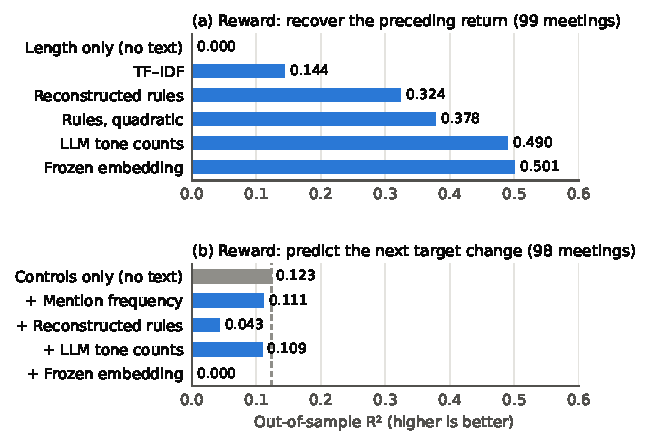
\includegraphics[width=\linewidth]{fig/reward_headroom.pdf}
\caption{Reward headroom. Out-of-sample $R^2$ of frozen readers under two candidate rewards; gray marks the no-text baseline. (a) Every text reader beats length alone when recovering the preceding return. (b) No text reader improves on the controls when predicting the next change in the policy rate.}
\label{fig:headroom}
\Description{Two horizontal bar charts. In panel a, out-of-sample R-squared rises from 0.000 for length only to 0.501 for the frozen embedding. In panel b, the no-text controls reach 0.123 and every text reader is at or below it, with the embedding at 0.000.}
\end{figure}

\textbf{Recovery has headroom.} Figure~\ref{fig:headroom}a shows that every text reader beats document length, and the LLM-based readers reduce MSE relative to the lexical rules by 18--26\%, depending on the reader and the rule specification. Against the quadratic rules the embedding reduces MSE by 19.9\%. Its advantage persists when the rules and the embedding see the same passages with a passage-count control (24.0\% relative to the matched rules) and under two alternative return definitions (26.0\% and 27.0\% against the quadratic rules). The gain is imprecisely estimated. The conditional 95\% block-bootstrap interval for the embedding against quadratic rules is $-3.6\%$ to 34.2\%, and no paired test survives a Holm adjustment. The five-category LLM tone counts come within 2.2\% of the 3,072-dimensional embedding in MSE, so a small, interpretable categorical action space keeps most of the learnable signal. This matters for harness adaptation, which edits the instructions that produce these categories.

\textbf{Policy prediction has no headroom.} We wrote the policy test (target, controls, representations, splits, five contrasts, and inference) into a protocol and hashed it before computing any estimate. Earlier in-sample analyses had already related minutes language to policy when we wrote the protocol. Figure~\ref{fig:headroom}b and Table~\ref{tab:policy} show the result. The no-text controls reach an out-of-sample $R^2$ of 0.123. Adding LLM tone counts raises MSE by 1.5\%, the rules by 9.1\%, and the embedding by 14.0\%. Every interval includes zero and every Holm-adjusted $p$ equals 1.00. The conclusion survives restricting the controls to information available at the meeting. Two sensitivities show weak signal. When the target counts only the change decided at the next meeting, which excludes rate changes between meetings, the rules and LLM tone gain 7--9\% (unadjusted $p\approx0.08$). On the meetings shared with the original study, with evaluation starting in September 2007 (75 meetings, including the crisis easing), the embedding gains 9.8\% ($p=0.09$). Both are unadjusted secondary results. On this evidence, the equity discussion in the minutes, however well measured, adds little detectable information to what returns and the policy state already say about the next decision.

\begin{table}[t]
\caption{Policy reward screen: next-cycle change in the target rate, 98 evaluation meetings. RMSE is in basis points. MSE reduction is relative to the no-text controls, so negative values mean higher error; brackets give a conditional 95\% block-bootstrap interval (block length 4, 9,999 draws). Mention frequency was not a pre-specified contrast.}
\label{tab:policy}
\small
\begin{tabular}{@{}lrrl@{}}
\toprule
Reader added to controls & RMSE & OOS $R^2$ & MSE reduction \\
\midrule
None (controls only) & 24.85 & 0.123 & -- \\
Mention frequency & 25.01 & 0.111 & $-1.3\%$ \\
Reconstructed rules & 25.96 & 0.043 & $-9.1\%$ [$-22.7$, 5.7] \\
LLM tone counts & 25.04 & 0.109 & $-1.5\%$ [$-10.5$, 17.7] \\
Frozen embedding & 26.53 & 0.000 & $-14.0\%$ [$-27.5$, 11.6] \\
\bottomrule
\end{tabular}
\end{table}

\textbf{Release reactions have no headroom out of sample.} An earlier exploratory screen used the frozen embedding to predict returns after the release of the minutes, on chronologically held-out meetings. It found negative out-of-sample $R^2$ at every horizon from one minute ($-0.157$) to five days ($-0.020$). In-sample regressions from the same exploratory work, which selected the best of many specifications, had reported sizable fits at these horizons. An adaptation loop that keeps whichever instruction wins on a small validation set would find gains of that kind and store them.

\textbf{Implication.} By Eq.~\eqref{eq:headroom}, recovery has headroom $H=0.50$ over document length, while the policy reward has $H<0$; every reader does worse than the controls alone. In this sample, only recovery gives an adaptation loop something to learn, and the policy and release-reaction rewards would teach it to overfit.

\section{Credit assignment: large residuals on correctly signed labels}\label{sec:credit}

We ran the first stage of an adaptive-reader pilot on the training window of fold 0. A frozen LLM reader (\texttt{gemini-3.8-flash}, fixed instructions) classified 253 calibration passages from 60 meetings and 117 feedback passages from the next 20. All 370 responses pass format checks, and every cited quotation appears verbatim in its passage. We did not measure semantic accuracy. The calibrated readout (penalty 1.0) has training MSE 11.92, inner-validation MSE 14.69, and feedback MSE 40.11.

\begin{table}[t]
\caption{Pilot feedback episodes with the largest squared errors (fold 0). Target and estimate are returns in percentage points. SSE share is the episode's share of the sum of squared errors over the 20 feedback episodes.}
\label{tab:credit}
\small
\begin{tabular}{@{}lrrr@{}}
\toprule
Meeting & Target & Estimate & SSE share \\
\midrule
Oct 29, 2008 & $-30.99$ & $-5.77$ & 79.3\% \\
Apr 30, 2008 & 7.14 & 0.57 & 5.4\% \\
Jun 25, 2008 & $-6.96$ & $-0.69$ & 4.9\% \\
Jun 24, 2009 & 2.27 & 6.69 & 2.4\% \\
Aug 5, 2008 & $-1.96$ & $-6.23$ & 2.3\% \\
\bottomrule
\end{tabular}
\end{table}

Table~\ref{tab:credit} shows that one episode dominates the feedback. It is the October 2008 meeting, whose intermeeting window spans the post-Lehman crash. The reader labeled all five of its passages negative, the correct direction for a $-31$ percentage-point intermeeting return. The error comes from magnitude. The target lies far below the calibration range ($-18.3$ to $+9.9$), and a count-based readout cannot express ``much more negative than usual.'' A reflector given the largest residuals sees a large error on text labeled in the correct direction. It is therefore invited to change labels or definitions to fit a magnitude its action space cannot represent. Figure~\ref{fig:example} shows why the labels cannot carry the magnitude. The minutes describe the crash in words that also describe ordinary declines. Across the corpus, the same strong-decline wording accompanies preceding returns from $-31.0$ to $+6.7$ percentage points. Labels elsewhere in the feedback set may still be wrong, and a residual cannot say which passage, if any, was misread.

\begin{figure}[t]
\small
\fbox{\parbox{0.95\linewidth}{\raggedright
\textbf{Meeting of October 29, 2008} \hfill target $-31.0$ pp; estimate $-5.8$ pp\\[2pt]
\emph{``Broad equity price indexes declined sharply over the intermeeting period, and option-implied volatility on the S\&P 500 index rose well above its previous record high.''} $\rightarrow$ negative\\[2pt]
\emph{``Equity prices had varied widely and were substantially lower, on net.''} $\rightarrow$ negative\\[2pt]
All five passages are labeled negative. The same strong-decline wording (``declined sharply,'' ``steep declines,'' ``substantially lower'') appears in the equity passages of 33 meetings whose preceding returns range from $-31.0$ to $+6.7$ pp (median $-5.0$).}}
\caption{Excerpts from the episode that dominates the pilot's feedback error . The reader's direction labels are correct, and the text gives no numerical magnitude.}
\label{fig:example}
\Description{A boxed excerpt of two sentences from the October 2008 FOMC minutes, each labeled negative, with the target and estimated returns and a note that similar wording appears in 33 meetings with widely different returns.}
\end{figure}

The case is a financial analogue of the gap between outcome and process supervision~\cite{uesato2022process,lightman2024verify}. We draw three design consequences. First, feedback should separate direction errors from magnitude errors, for example by comparing the reader's categories with a direction-only check before exposing residuals. Second, the action space should include an intensity channel if the target rewards magnitude. Third, an edit should persist in memory only if it lowers the error on held-out gate meetings, so that fitting one extreme feedback episode cannot by itself change the reader.

The pilot also produced five instruction proposals from an outcome-blind proposer and one 367-word proposal from a reflector shown the six largest feedback errors. Several blind proposals raise the same ideas as the reflector's proposal (time horizons, net versus gross movement), so blind search is a substantive control. None of these candidates has been scored.

\section{Adaptation protocol and its cost}\label{sec:protocol}

\begin{figure}[t]
\centering
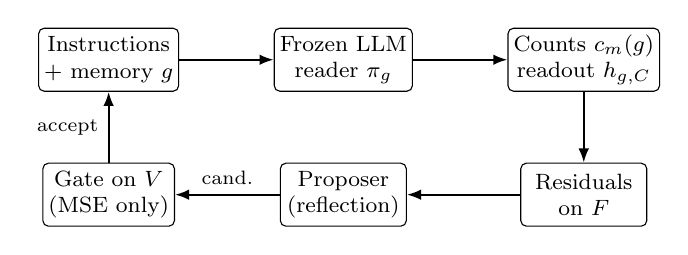
\begin{tikzpicture}[font=\footnotesize, node distance=5mm and 12mm, box/.style={draw, rounded corners=2pt, align=center, minimum height=8mm, minimum width=16mm, inner sep=2pt}, arr/.style={-{Latex[length=1.8mm]}, thick}]
\node[box] (g) {Instructions\\+ memory $g$};
\node[box, right=of g] (r) {Frozen LLM\\reader $\pi_g$};
\node[box, right=of r] (a) {Counts $c_m(g)$\\readout $h_{g,C}$};
\node[box, below=9mm of a] (s) {Residuals\\on $F$};
\node[box, below=9mm of r] (p) {Proposer\\(reflection)};
\node[box, below=9mm of g] (v) {Gate on $V$\\(MSE only)};
\draw[arr] (g) -- (r); \draw[arr] (r) -- (a); \draw[arr] (a) -- (s); \draw[arr] (s) -- (p);
\draw[arr] (p) -- node[above, font=\scriptsize]{cand.} (v);
\draw[arr] (v) -- node[left, font=\scriptsize]{accept} (g);
\end{tikzpicture}
\caption{Validation-gated harness adaptation. Only the instructions and memory $g$ change. The proposer sees residuals on the feedback meetings $F$, and the gate on $V$ returns only accept or reject. The evaluation block $E$ is scored once, after all artifacts are fixed.}
\label{fig:loop}
\Description{A loop diagram: instructions and memory feed a frozen LLM reader, whose counts go to a readout; feedback residuals go to a proposer, whose candidate is checked by a validation gate that decides whether it persists. A note describes the calibration, feedback, gate, and evaluation roles.}
\end{figure}

\begin{table}[t]
\caption{Adaptation arms. All arms share the reader model, proposal budget, 400-word memory limit, five-category ontology, and calibration-only readout.}
\label{tab:arms}
\small
\begin{tabular}{@{}p{0.27\linewidth}p{0.3\linewidth}p{0.33\linewidth}@{}}
\toprule
Arm & Proposer sees & Persistence \\
\midrule
Fixed instructions & -- & -- \\
Blind search & Task description only & Gate on $V$ with margin \\
Ungated reflection & Largest $F$ residuals & Every valid candidate \\
Gated reflection & Largest $F$ residuals & Gate on $V$ with margin \\
\bottomrule
\end{tabular}
\end{table}

\textbf{Roles.} Within each outer training window, the oldest 60\% of meetings calibrate the readout ($C$), the next 20\% supply reflection feedback ($F$), and the newest 20\% form the gate ($V$). The outer evaluation block ($E$) never enters the loop. In the reflection arms the proposer sees only the residuals on $F$. The evaluation harness scores candidates on $V$ and returns only an accept or reject decision to the proposer.

\textbf{Arms.} Table~\ref{tab:arms} lists the four arms: a fixed-instruction reader, outcome-blind prompt search, ungated reflection, and validation-gated reflection (Figure~\ref{fig:loop}). Each candidate relabels $C$ and refits its own readout. In the gated arms (blind search and gated reflection), a candidate persists only if it beats the incumbent's gate MSE by a fixed margin with all outputs valid. The primary estimand is the paired evaluation-MSE difference between gated reflection and fixed instructions. Blind search isolates the value of feedback, and ungated reflection the value of gating.

\textbf{The cost of role separation.} Reserving $F$ and $V$ removes 40\% of the training meetings from calibration. Refitting the frozen readers under this rule raises the embedding's RMSE from 3.522 to 3.788, a 15.7\% increase in MSE, while the linear rules barely move (4.100 to 4.086). An adaptive arm must recover this loss to match a fully calibrated reader, so the fair baseline is a fixed reader under the same calibration-only rule; for the embedding, that baseline has RMSE 3.788.

\textbf{Minimal next run.} Completing one fold requires 771 additional passage classifications for a single-proposal comparison of the fixed-instruction, ungated, and gated arms, or 1,283 with a matched blind proposal. Evidence of transfer requires unseen documents and a fixed endpoint.

\section{A reward checklist for financial reading agents}

We suggest five checks before launching any adaptive loop.

\textbf{1. Measure headroom with frozen readers.} Compute Eq.~\eqref{eq:headroom} for the candidate reward on untouched evaluation data. Here it separates a usable reward (recovery, $H=0.50$) from the policy reward ($H<0$) at the cost of a few ridge fits, and an exploratory screen gave negative out-of-sample $R^2$ for release reactions.

\textbf{2. Fix the reward before estimation.} Write down and hash the target, controls, splits, contrasts, and inference before estimation, as we did for the policy test, and preferably before any exploratory look at the outcome. In-sample fits chosen from many specifications looked promising for release reactions and did not survive out of sample.

\textbf{3. Check concentration.} Rare episodes can dominate squared-error rewards. One meeting produces 79\% of the pilot's feedback error, and three policy cycles produce 45\% of the controls-only error on the policy task. Robust losses, per-episode caps, or error sampling stratified by regime would make the feedback more representative of the whole task.

\textbf{4. Separate reading from calibration.} If an action space cannot express a quantity the reward depends on, here magnitude, route the feedback to the readout or to a new action channel and leave the labels unchanged.

\textbf{5. Charge the cost of held-out roles.} Compare an adaptive arm with a fixed reader that loses the same meetings from calibration, here a 15.7\% rise in MSE.

\section{Limitations}

The benchmark covers one document type from one central bank, with 99 evaluation meetings (35 overlapping the human-coded references) and 27 target-rate changes among the 98 policy evaluation meetings. All splits come from a historical corpus that informed earlier model and outcome choices, and the bootstrap intervals condition on that search. The recovery target is a price-return proxy that omits dividends, and the human-coded references are approximations recovered from published figures. We verified the pilot's reader outputs for format and evidence only, and no adaptive arm has been evaluated.

\section{Conclusion}

Outcome-guided agents in finance need rewards that the text can explain. On a verified FOMC benchmark, recovering the market's preceding move is such a reward. Frozen LLM readers reduce error relative to the reconstructed lexical rules, though imprecisely, and come close to human coding on the 35 evaluation meetings that the human-coded sample covers. Rewards based on the next policy decision or on the market's reaction to the release do not pass the headroom test. A single crisis episode shows why residual-driven reflection is risky even with a good reward. Large errors can fall on passages labeled in the correct direction, so feedback must separate reading from calibration, and an edit must pass a held-out gate before it persists. We release the environment, comparators, hashed policy protocol, and pilot artifacts so that the adaptation arms can be run against these baselines.

\section*{Artifact availability}
Code and data are available at\newline \url{https://github.com/ginolatino32/fomc-reward-benchmark}. The repository contains the minutes with source hashes, the reconstructed rules and their tests, the recovered human-coded series, the frozen representations and predictions, the hashed policy protocol, and the pilot's reader outputs and proposals. S\&P 500 prices are not redistributed; a script downloads them.

\bibliographystyle{ACM-Reference-Format}
\bibliography{refs}

\end{document}
